% peer_poll.tex
\chapter{Peer/Poll Processes}
\label{cha:peer/poll}

\section{Concepts}%
\label{sec:peer/poll_concepts}
\begin{enumerate}
    \item Offset $\theta$\\
        The maximum-likelihood time offset of the server clock relative to the
        system clock. This concept describes how different the client's time
        and the server's time are.
        % $$\theta_{AB} = \frac{1}{2}\left[\left(T_{i-2} - T_{i-3}\right) +
        % \left(T_{i-1} - T_i\right)\right]$$
    \item Delay $\delta$\\
        The round-trip delay between the client and server. It is equal to the
        time that a massage travels from the client to the server and the time
        it comes back.
        % $$\delta_{AB} = \left(T_{i} - T_{i-3}\right) - \left(T_{i-1} -
        % T_{i-2}\right)$$
    \item Dispersion $\varepsilon$\\
        The maximum error inherent in the measurement.
        Another definition: Potential clock offset error due to the maximum
        uncorrected system clock frequency error.
        These definitions are in some respect confused, we will discuss it with
        more detail in Section~\ref{sec:peer_processes}.
        % from website https://www.eecis.udel.edu/~mills/ntp/html/stats.html
\end{enumerate}

\section{Overview}%
\label{sec:peer_poll_overview}
Figure~\ref{fig:peer_poll_processes} shows the basic architecture of peer/poll
processes. The communication between client and server uses on-wire protocol,
which can provide sample statistics ($\theta_0, \delta_0, t_0$ in the figure).
The recent eight samples are stored in a shift register, with one more sample
statistic added ($\varepsilon$).  Then peer process applies clock filter
algorithm, which generates peer statistics ($\theta, \delta, \varepsilon,
\varphi$ in the figure), and passes them to system process.


% figures/peer_poll_figure.tex

\begin{figure}[htpb]
\begin{center}
\begin{tikzpicture}[scale=0.7, transform shape,
        squarednode/.style={rectangle, draw=black, very thick, minimum
        size=10mm, minimum width=20mm, align=center},
        border/.style={draw=black, dashed, very thick},
    ]
    % Nodes
    % server
    \node[squarednode]  (s)                {Server};

    % on-wire protocol
    \node[align=center] (onwire) at ($(s.east) + (2.5, 2)$) {On-wire Protocol};
    \draw[border] ($(onwire.north west) + (-0.2, 0.2)$) -|
            ($(onwire.north east) + (0.2, -5)$) -|
            ($(onwire.north west) + (-0.2, 0.2)$);
    % poll process
    \node[squarednode] (poll) at ($(onwire) + (0, -6)$) {Poll Process};
    \draw[-latex, thick] (poll) |- ($(s.south) + (0, -0.5)$) -- (s);

    % shift registers
    \node[squarednode] (sr) at ($(onwire) + (4.5,-2)$) 
            {Shift Registers\\
            $(\theta_1, \delta_1, \varepsilon_1, t_1)$\\
            $(\theta_2, \delta_2, \varepsilon_2, t_2)$\\
            $(\theta_3, \delta_3, \varepsilon_3, t_3)$\\
            $(\theta_4, \delta_4, \varepsilon_4, t_4)$\\
            $(\theta_5, \delta_5, \varepsilon_5, t_5)$\\
            $(\theta_6, \delta_6, \varepsilon_6, t_6)$\\
            $(\theta_7, \delta_7, \varepsilon_7, t_7)$\\
            $(\theta_8, \delta_8, \varepsilon_8, t_8)$
            };
    \draw[-latex, thick] (s) -- (sr) node[midway, above] 
            {$(\theta_0, \delta_0, t_0)$};
    % clock filter algorithm
    \node[squarednode] (cf) [right=of sr] {Clock Filter\\ algorithm};
    \draw[-latex, thick] (sr) -- (cf);

    % peer process
    \node[align=center] (peer) [below=2mm of sr.south east] {Peer Process};
    \draw[border] ($(sr.north west) + (-0.5, 0.2)$) -- 
            ($(sr.south west) + (-0.5, -1.2)$)
            -|
            ($(cf.east) + (0.2, 0)$) |-
            ($(sr.north west) + (-0.5, 0.2)$);


    % system process
    \node[squarednode] (sp) [right=2.5 of cf] {System process};
    \draw[-latex, thick] (cf) -- (sp) node[midway, above] 
            {$(\theta, \delta, \varepsilon, \varphi)$};
    
    % synchronizations
    % \draw[-latex, ultra thick] (s1) -- (rc);

\end{tikzpicture}
\end{center}
\caption{Peer/Poll processes}
\label{fig:peer_poll_processes}
\end{figure}



% fig:peer_poll_processes

The purpose of peer processes is to communicate with servers and to keep
statistics of the communications which can be used to determine how reliable
the servers are. And for poll processes, their job is to manage the
communications to get sufficient data without making the servers too busy.

\section{On wire protocol}%
\label{sec:on_wire_protocol}
In NTP subnet, a client can send request to server and the server sends back
response after it got the request. The whole round of the communication can
generate a sample. For every sample, the client wants to know the difference
between the server's system clock and its, aka offset.
But it may take a while for the server to give the response. And it is not
predictable, as well as the network delay between the two devices.
In NTP subnet, clients and servers communicate under on-wire protocol. It
provides a smart way to calculate offset and delay for every sample. 

\subsection{Statistics calculation}%
\label{sub:statistics_calculation}
Figure~\ref{fig:on_wire1} represents the timestamps and communications between
a client and a server. The vertical dash line indicates the same time. The
arrow indicates the communication packets sent from one side and received at
the other side. The notation $T_i$ stands for the timestamp gotten from the
system clock of one device. 

% figures/on_wire1.tex

\begin{figure}[htpb]
\begin{center}
\begin{tikzpicture}[scale=0.7, transform shape,
        textnode/.style={rectangle, very thick, minimum
        size=10mm, minimum width=20mm, align=center},
        border/.style={draw=black, dashed, very thick},
        arrow/.style={-latex, ultra thick},
    ]
    % server
    \node[textnode]  (s)                {Server};
    \draw[arrow]     (s) -- ($(s) + (10,0)$);

    % client
    \node[textnode]  (c)    [below=20mm of s]            {Client};
    \draw[arrow]     (c) -- ($(c) + (10,0)$);

    % communications
    \draw[arrow]     ($(c) + (5, 0)$) -- ($(s) + (6, 0)$);
    \draw[arrow]     ($(s) + (8, 0)$) -- ($(c) + (9, 0)$);

    % vertical line
    \draw[border]    ($(s) + (3, 1)$) -- ($(c) + (3, -1)$);

    % labels
    \node[textnode] at ($(c) + (2.5, -0.5)$)   {$t_0$};
    \node[textnode] at ($(s) + (2.5, 0.5)$)    {$t_1$};
    \node[textnode] at ($(c) + (5, -0.5)$)   {$t_2$};
    \node[textnode] at ($(s) + (6, 0.5)$)    {$t_3$};
    \node[textnode] at ($(s) + (8, 0.5)$)    {$t_4$};
    \node[textnode] at ($(c) + (9, -0.5)$)   {$t_5$};

\end{tikzpicture}
\end{center}
\caption{Time stamps}
\label{fig:on_wire1}
\end{figure}



% fig:on_wire1

In ideal situation, if we have $T_1$ and $T_0$, which are timestamps gotten
from both devices at the same time, then we can get the offset $\theta$:
$$\theta = T_1 - T_0$$
But we cannot do this since we cannot determine whether two timestamps were
token at the same time. The on-wire protocol actually calculates the offset in
an alternative way:
\begin{equation}
    \theta = \frac{1}{2}\left[(T_3 - T_2) + (T_4 - T_5)\right]
    \label{eq:offset_def}
\end{equation}
Note that this equation is equivalent to:
$$\theta = \frac{T_3 + T_4}{2} - \frac{T_2 + T_5}{2}$$
which means that the offset is equal to the difference between two timestamps
which are the middle points of $T_3, T_4$ and $T_2, T_5$. 
If the network delay is symmetric, which means the time for packets to travel
from client to server and the time for packets to get back are equal, the
middle points are at the same time. In this case, it is equivalent to the ideal
situation. If the delay is asymmetric, there will be an error of the
calculation. This error is impossible to be corrected. However, there is one
scenario that the error can be attenuated.~\cite{redbook} We will discuss this
part in Section~\ref{sub:huff_n_puff_filter}.

The delay $\delta$ is calculated by:
\begin{equation}
    \delta = (T_5 - T_2) - (T_4 - T_3)
    \label{eq:delay_def}
\end{equation}
It is actually a difference of two time periods. It is not impacted by the
offset, since each time period is calculated using two timestamps from the same
device.
(NOTE: add the impact of frequency offset.)

There is another statistic $t$ in Figure~\ref{fig:peer_poll_processes}, which
indicates the time that the offset $\theta$ and delay $\delta$ are calculated.
In practice we can let $t = T_5$, because it is just used to indicate the order
of groups of sample statistics, we do not need it to be extremely accurate.
It is maintained by clock-adjust process. It counts the seconds since the
service was started.
In Figure~\ref{fig:peer_poll_processes}, we add subscript 0 to distinguish the
new group of samples statistics and the groups which are in the shift register.

\subsection{Timestamps in NTP packet}%
\label{sub:timestamps_in_ntp_packet}
% how to store timestamps and modes
% https://www.eecis.udel.edu/~mills/onwire.html
NTP uses NTP packets in communications. The NTP packet is a UDP
datagram.~\cite{rfc5905} There are four timestamps in NTP packet header:
\begin{enumerate}
    \item Reference Timestamp\\
        Time when the system clock was last set or corrected.
    \item Origin Timestamp (\emph{org})\\
        Time at the client when the request packet departs from it.
    \item Receive Timestamp (\emph{rec})\\
        Time at the server when the request packet is receive by it.
    \item Transmit Timestamp (\emph{xmt})\\
        Time at the server when the response packet departs from it.
\end{enumerate}
In peer process, we are interested in another one: destination
timestamp(\emph{dst}), which is the time at the client when it receives the
response packet. And the reference timestamp is not interested here. In
Figure~\ref{fig:on_wire1}, the packet leave at $T_4$ contains $T_4, T_3$ and
$T_2$ in its header, where
$$ org = T_2,~rec = T_3,~xmt = T_4 $$
When the client gets the packet, it captures $dst = T_5$.

The purpose of on-wire protocol is to calculate offset $\theta$ and delay
$\delta$ based on the communication. The four timestamps used in
Equation~\ref{eq:offset_def} and Equation~\ref{eq:delay_def} are important,
which are \emph{org}, \emph{rec}, \emph{xmt} and \emph{dst}.
High accuracy requires that they are captured as close to the actual time of
the relative event (sending or receiving packet) as possible. On-wire protocol
provides two interleaved modes which are \emph{interleaved symmetric} and
\emph{interleaved broadcast}. They are extensions of basic symmetric mode and
basic broadcast mode.~\cite{on_wire} 
%
In basic modes, \emph{org} and \emph{xmt} in outgoing packet are captured
before the packet is made, which is not the timestamp when the packet is sent. 
This kind of timestamps are called \emph{softstamps}. In this case, 
after softstamp is captured, there are something else to do before sending the
packet, such as add validation information to the packet and adding the packet
to the output queue, then the packet will wait in the queue before it is sent.
For \emph{rec} and \emph{dst}, which are also called \emph{drivestamps}, they
are captured ``shortly after the input device interrupt and before adding the
buffer to the input queue''.\cite{on_wire} We can see that the drivestamps are
more accurate than softstamps because there is only a short delay by handling
the interrupt. If we can capture timestamps exactly when packets are sent or
received, they will be more accurate. However, we need additional hardware
support to do this.

In interleaved modes, we can make softstamps more accurate without
additional hardware support. The trade off is that we need more packets.
Instead of capturing softstamps before the packets are made, we can capture
them shortly after the output interrupt. In this case, the accuracy is similar
with drivestamps but they can not be sent in the very packets which they
represent the time they are sent. We need one more packet if we want to send
softstamps. More detail about interleaved modes are beyond the scope of this
thesis.

\subsection{Non-reliable protocol}%
\label{sub:non_reliable_protocol}
As mentioned in Section~\ref{sub:timestamps_in_ntp_packet}, the NTP packet is a
UDP datagram. This make on-wire protocol not reliable, which means that there
is no guarantee about the packet. Reliable delivery actually decreases the
reliability of NTP packet. Assume we are implementing on-wire protocol to make
it reliable by using similar technique like TCP, a lost packet will be sent
again. However, an identical packet is not valid since the timestamp which
indicates the time when the packet is sent is incorrect.

\section{Peer processes}%
\label{sec:peer_processes}
For each server, on-wire protocol provides sample statistics $\theta, \delta$
and $t$ and passes them to peer process. Then the peer process maintains them
and the clock filter algorithm calculates peer statistics based on them.

\subsection{Sample statistics maintenance}%
\label{sub:sample_statistics_maintenance}
As mentioned in Section~\ref{sec:peer_poll_overview}, there is a shift register
which stores the recent eight samples. When a packet arrives, the peer process
replace the oldest sample by the new one with a dispersion $\varepsilon$ added.
The dispersion is initialized as:
$$ \varepsilon = \rho_r + \rho_s + \phi (T_5 - T_2) $$
Where 
\begin{itemize}
    \item 
        $\rho_r$ is the root precision in NTP packet. 
    \item 
        $\rho_s$ is the system
        precision which we will discuss in next chapter. (NOTE: REF HERE).
    \item
        $\phi = 15 ppm = 15 \mu s/s$ is a constant.
    \item
        $T_5$ and $T_2$ are the two timestamps in Figure~\ref{fig:on_wire1}. In
        other word, $T_5$ is \emph{dst} and $T_2$ is \emph{org}.
\end{itemize}
After storing the sample statistics into the shift register, the peer process
increases dispersion in a constant rate $\phi$.

In Section~\ref{sec:peer/poll_concepts} we mentioned that dispersion is the
maximum error. Now we can consider dispersion as a function of time ($t$) and
we have:
\begin{equation}
    \varepsilon(t) = \rho_r + \rho_s + \phi (t - T_2)
    \label{eq:dispersion}
\end{equation}
In Equation~\ref{eq:dispersion}, dispersion has two parts. $\rho_r + \rho_s$
represents the error due to the precisions of server and client clocks. $\phi
(t - T_2)$ represents the error due to frequency tolerance and time.
(TODO: add more about 15 ppm)

\subsection{Initial and invalid samples}%
\label{sub:initial_and_invalid_samples}
When the service starts, all eight samples in the shift register are
initialized to the dummy tuple: $\theta = 0, \delta = MAXDISP, \varepsilon =
MAXDISP, t = 0$, where $MAXDISP = 16$ is the maximum dispersion.~\cite{rfc5905} 

There is a 8-bit shift register called reach register which is shared by peer
and poll process and used to determine whether the server is reachable and the
data is fresh. It is maintained by poll process, which we will discuss in
Section~\ref{sec:poll_processes}. After a packet is sent to the server, the
register is shifted left by one bit and the rightmost bit is set to 0. If a
valid packet is arrived from the server, the rightmost bit is set to 1. A
server is reachable only when there is at least one non-zero bit in the
register. If the three rightmost bit are all 0, there will be a dummy tuple
inserted into the shift register of samples by replacing the oldest one which
indicates invalid sample.

\subsection{Clock filter algorithm}%
\label{sub:clock_filter_algorithm}
The clock filter algorithm calculates peer statistics used in system process.
As mentioned in Section~\ref{sec:peer_poll_overview}, there are 8 samples in
the shift register. Clock filter algorithm selects one of them represents the
offset and delay of the server, then calculates the dispersion and jitter,
passes them to the system process as well as the arrive time of selected
sample.

Figure~\ref{fig:clock_filter} is ``a wedge scattergram plotting sample points of
offset versus delay collected over a 24-hr period''. (NOTE: cite here) It shows
that with as the delay increases, the variance of offset increases as well. In
this case, the best sample should be the one with lowest delay.

% clock_filter

\begin{figure}[htb]
    \centering
    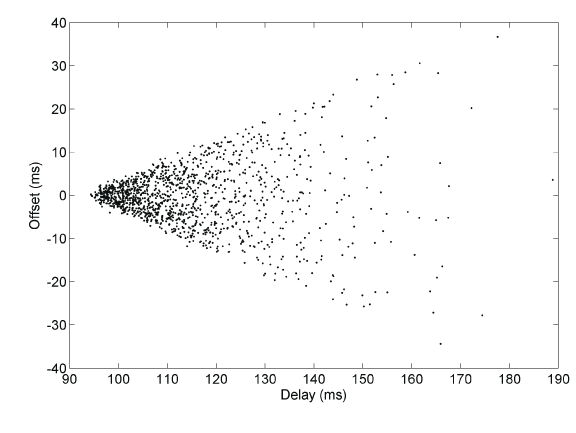
\includegraphics[width=0.5\textwidth]{figures/clock_filter.png}
    \caption{Wedge Scattergram}
    \label{fig:clock_filter}
\end{figure}


% fig:clock_filter

Based on the result we got from Figure~\ref{fig:clock_filter}, clock filter
algorithm first sort the samples by their delay. If the first sample is later
than the last sample we chose, it is selected, otherwise nothing more happen.
This mechanism guarantees that one sample will only be used at most once.

After the selection, the offset $\theta$ and delay $\delta$ of the sample
become peer statistics with the same names. The sorted samples are indexed from
0 to 7 from the one with the lowest delay to the one with highest. Here
$\varepsilon_i$ indicates the dispersion of the sample with index $i$. We
calculate peer dispersion $\varepsilon$ by:
\begin{equation}
    \varepsilon = \sum^{7}_{i=0} \frac{\varepsilon_i}{2^{(i+1)}}
    \label{eq:peer_dispersion}
\end{equation}
The peer jitter $\varphi$ is calculated by:
\begin{equation}
    \varphi = \sqrt{\frac{1}{n-1} \sum^{n-1}_{j=1} (\theta_0 - \theta_j)^2}
    \label{eq:peer_jitter}
\end{equation}
where $n$ is the number of valid samples in the shift register ($n > 1$).
The peer jitter is the root mean square (RMS) of difference between sample
offsets and the sample offset of selected sample. A larger jitter indicates
that the offset varies more, which we can consider that there may be some
problem with the server and/or the connection, since the offset should not
change much if we did not adjust client's system clock by a large amount.

\subsection{Huff-'n-puff filter}%
\label{sub:huff_n_puff_filter}

%\subsection{Reachability detection}%
%\label{sub:reachability_detection}
% https://docs.ntpsec.org/latest/stats.html
% redbook

\section{Poll processes}%
\label{sec:poll_processes}


